\begin{figure}[ht!]
  \center
  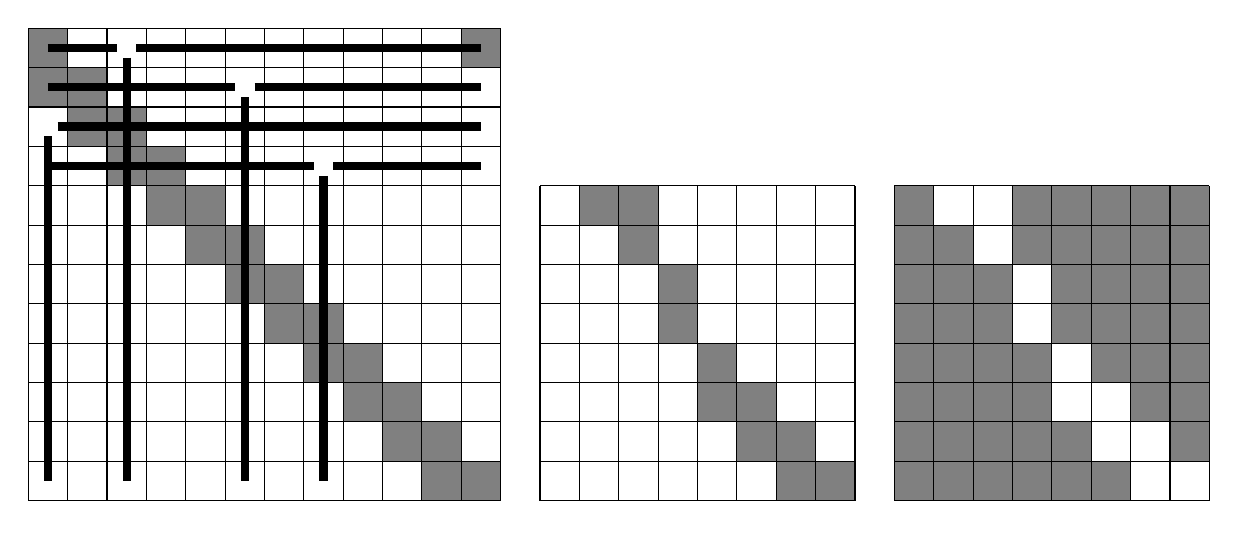
\begin{tikzpicture}[scale = 0.5]
    \path (0,-0.5) -- (0,6.5);
    \foreach \i in {0,...,11} { \fill[gray] (\i, 12-\i) rectangle (\i + 1, 11 - \i); }
    \foreach \i in {0,...,10} { \fill[gray] (\i, 11-\i) rectangle (\i + 1, 10 - \i); }
    \fill[gray] (11,11) rectangle (12,12);
    \draw (0,0) grid (12,12);
    \node (R1) at (2.5, 11.5) {\Large\symrook};
    \node (R2) at (5.5, 10.5) {\Large\symrook};
    \node (R3) at (0.5, 9.5) {\Large\symrook};
    \node (R4) at (7.5, 8.5) {\Large\symrook};
    \draw[line width = 3]
      (0.5,11.5) -- (R1) -- (11.5,11.5)
      (R1) -- (2.5,0.5)
    ;
    \draw[line width = 3]
      (0.5,10.5) -- (R2) -- (11.5,10.5)
      (R2) -- (5.5,0.5)
    ;
    \draw[line width = 3]
      (R3) -- (11.5,9.5)
      (R3) -- (0.5,0.5)
    ;
    \draw[line width = 3]
      (0.5,8.5) -- (R4) -- (11.5,8.5)
      (R4) -- (7.5,0.5)
    ;
    % ---------------------------------------------
    \foreach \i/\j in {1/7, 2/6, 2/7, 3/4, 3/5, 4/2, 4/3, 5/2, 5/1, 6/1, 6/0, 7/0} {
      \fill[gray, xshift=13cm] (\i, \j) rectangle (\i + 1, \j + 1);
    }
    \draw[xshift=13cm] (0,0) grid (8,8);
    % ---------------------------------------------
    \fill[xshift=22cm, gray] (0,0) rectangle (8,8);
    \foreach \i/\j in {1/7, 2/6, 2/7, 3/4, 3/5, 4/2, 4/3, 5/2, 5/1, 6/1, 6/0, 7/0} {
      \fill[white, xshift=22cm] (\i, \j) rectangle (\i + 1, \j + 1);
    }
    \draw[xshift=22cm] (0,0) grid (8,8);
  \end{tikzpicture}
  % ~~~
  % \begin{tikzpicture}[scale = 0.5]
  %   \path (0,-0.5) -- (0,6.5);
  %   \foreach \i/\j in {0/7, 0/6, 1/6, 1/5, 2/5, 2/4, 3/4, 4/3, 5/3, 5/2, 6/1, 6/0} {
  %     \fill[gray] (\i, \j) rectangle (\i + 1, \j + 1);
  %   }
  %   \draw (0,0) grid (8,8);
  %   \draw[ultra thick, dashed, red]
  %     (0,8) rectangle (4,4)
  %     (4,4) rectangle (6,2)
  %     (6,2) rectangle (8,0)
  %   ;
  % \end{tikzpicture}
  \caption{
    The prefix $\alpha = (3,6,1,8)$,
    the derived board $B_\alpha$, and
    the derived complementary board
    $B_\alpha^c = \mathcal{O}_3 \sqcup \mathcal{E}_2 \sqcup \mathcal{O}_7^\intercal$.
    There are $8062$ ways of placing eight nonattacking rooks on $B_\alpha$.
  }
  \label{fig:menageMultiplePlacement}
\end{figure}
